\subsection*{Question 1}
\textbf{Provide the barrier function. Explain how the barrier function is used to approximate the problem with the indicator function $I-$. Explain what happens when one of the inequality constraints approaches zero.}

$$
\phi(x) = -\sum_{i=1}^m \log(- f_i(x))
$$

When an inequality constraint approaches zero, the corresponding term in barrier function goes to infinity. The penalty for violating the constraint is thus very large, and prevents it from happening in our optimisation problem, making sure the solution is feasible.

\subsection*{Question 2}
\textbf{Provide the centrality condition. Consider an LP in inequality form and the hyperspace defined by its inequality constraints. For such a problem, sketch an example of centrality path and explain it.}

Centrality condition makes sure that the points are strictly feasible and there exists $\hat \nu \in \mathbb{R}^p$ such that

$$
0 = t \nabla f_0(x^*(t)) + \nabla \phi(x^*(t)) + A^\top \hat \nu
$$

For an LP in inequality form, $f_0(x) = c^\top x$, $f_1(x) = Ax-b$, the centrality condition can be written as: 

$$
t c + \nabla \phi(x^*(t)) = 0.
$$

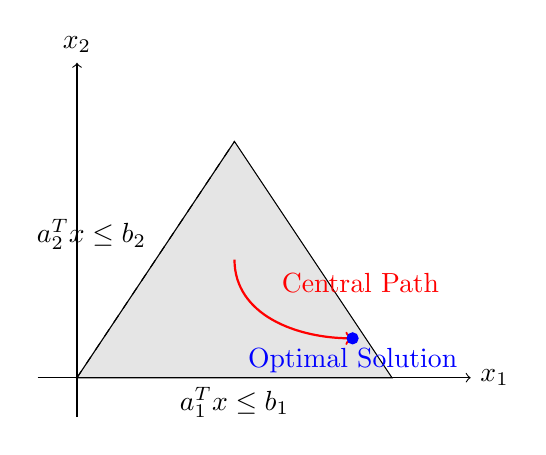
\begin{tikzpicture}
\filldraw[fill=gray!20, draw=black] (0,0) -- (4,0) -- (2,3) -- cycle;
\draw[thick, red, ->] (2,1.5) to[out=270, in=180] (3.5,0.5);
\node[red] at (3.6,1.2) {Central Path};
\filldraw[blue] (3.5,0.5) circle (2pt);
\node[blue, below] at (3.5,0.5) {Optimal Solution};
\draw[->] (-0.5,0) -- (5,0) node[right] {$x_1$};
\draw[->] (0,-0.5) -- (0,4) node[above] {$x_2$};
\draw[dashed] (0,0) -- (4,0) node[midway, below] {$a_1^T x \leq b_1$};
\draw[dashed] (0,0) -- (2,3) node[midway, above left] {$a_2^T x \leq b_2$};
\end{tikzpicture}


\subsection*{Question 3}
\textbf{Give the modified complementary condition associated to the centrality condition and explain it as a function of $t$.}

The modified complementary condition associated with the centrality condition is as follows:

$$
-\lambda_i f_i(x) = \frac{1}{t}, \quad i = 1, \dots, m.
$$

As \( t \) increases, the term \( \frac{1}{t} \) forces the complementary slackness to become smaller, and for large \( t \), the solution \( x^*(t) \) approaches the optimal point, the solution would satisfy the KKT conditions more closely. 


\subsection*{Question 4}
\textbf{Explain the differences between the two Phase I methods seen in the lecture.}

When the problem is infeasible, the maximum infeasibility method minimizes the largest constraint violation, the solutions we get in this way may have many constraints slightly violated.

The sum of infeasibilities method minimizes the total violation, most constraints are exactly satisfied, while a few may have larger violations.  

\subsection*{Question 5}
\textbf{Provide the duality gap associated to a convex optimisation problem with $m$ generalised inequalities which are $K_i$-convex and have generalised logarithms with degree $\theta_i$. Explain the role of $\theta_i$ in the computational complexity of the barrier method.}


The duality gap for a convex optimization problem with $m$ generalized inequalities, where each inequality is $K_i$-convex and has a generalized logarithm with degree $\theta_i$:

$$
\text{duality gap} = \frac {\sum_{i=1}^m \theta_i}{t}
$$

The generalized logarithm with degree $\theta_i$ ensures that the barrier function used to enforce the $K_i$-convex constraints has a self-concordant property. 